\documentclass[a4paper, UTF8]{ctexart}
%调整页边距
\usepackage{geometry}
%取消页首页眉编号
\pagestyle{empty}
%设置中文编号
\usepackage{CJKnumb}
\usepackage[bf, big, raggedright]{titlesec}
\titleformat{\section}{\bfseries\songti\zihao{4}}{\CJKnumber{\thesection}、}{0em}{}
%
\usepackage{tabularx}
\usepackage{booktabs}
\usepackage{setspace}
\usepackage{pdfpages}
%For empty line
\newcommand{\FirstSpace}{\vspace{33pt}}
\newcommand{\SecondSpace}{\vspace{55.5pt}}
\newcommand{\NormalSpace}{\vspace{35pt}}
\newcommand{\LastSpace}{\vspace{30pt}}
%Font set
\newenvironment{TitleFont}{\songti \zihao{2} \bfseries}{}
\newenvironment{NormalFont}{\songti \zihao{4} \bfseries}{}
\newenvironment{LastFont}{\songti \zihao{-4} \bfseries}{}
%To print table
\newcolumntype{Y}{>{\centering\arraybackslash}X}
%Print a normal line
\newcommand{\NormalRow}[2]{
	\begin{tabularx}{\textwidth}{cY}
		#1:& #2 \\
		\cmidrule{2-2}
	\end{tabularx}
}
%Print a line with 3 items
\newcommand{\ThreeRow}[6]{
	\begin{tabularx}{\textwidth}{cccccY}
		#1: & #2 & #3: & #4 & #5: & #6 \\
		\cmidrule{2-2} \cmidrule{4-4} \cmidrule{6-6}
	\end{tabularx}
}
\newenvironment{Cover}{
	%Infact in Word it is [top=2.54cm, bottom=2.54cm, left=3.17cm, right=3.17cm]
	\newgeometry{top=2.54cm, bottom=2.54cm, left=4.45cm, right=4.45cm}
}{}


\begin{document}
%------------------------------------------------
%首页
	%Infact in Word it is [top=2.54cm, bottom=2.54cm, left=3.17cm, right=3.17cm]
	\newgeometry{top=2.54cm, bottom=2.54cm, left=4.45cm, right=4.45cm}

	\phantom{blank}
	
	\FirstSpace
	
	\begin{TitleFont}
		\centering
		\newcommand{\TempSpace}{\hspace{0.1em}}
		\begin{tabularx}{\textwidth}{Y}
			深 \TempSpace 圳 \TempSpace
			大 \TempSpace 学 \TempSpace
			实 \TempSpace 验 \TempSpace
			报 \TempSpace 告 \\
		\end{tabularx}
	\end{TitleFont}
	
	\SecondSpace
	
	\begin{NormalFont}
		\centering	
		
		\NormalRow{课程名称}{未知} \\
		\NormalSpace
		\NormalRow{实验项目名称}{未知} \\
		\NormalSpace
		\NormalRow{学院}{未知} \\
		\NormalSpace
		\NormalRow{专业}{未知} \\
		\NormalSpace
		\NormalRow{指导教师}{未知} \\
		\NormalSpace
		\ThreeRow{报告人}{某某某}{学号}{2000000000}{班级}{00} \\
		\NormalSpace
		\NormalRow{实验时间}{1000年00月00日} \\
		\NormalSpace
		\NormalRow{实验报告提交时间}{1000年00月00日} \\
	\end{NormalFont}
	
	\LastSpace
	
	\begin{LastFont} \hspace{9em} 教务部制 \end{LastFont}
%------------------------------------------------
%正文部分
	\newpage
	\newgeometry{top=2.54cm, bottom=2.54cm, left=3.17cm, right=3.17cm}
	\CJKindent
	\songti \zihao{5}
	%
	\section{实验目的}
	
	\section{实验步骤与结果}
	
	\section{实验分析}
	
	\section{思考题}
	
	\section{实验心得}
	
%%------------------------------------------------
%教师评测部分
	\newpage
	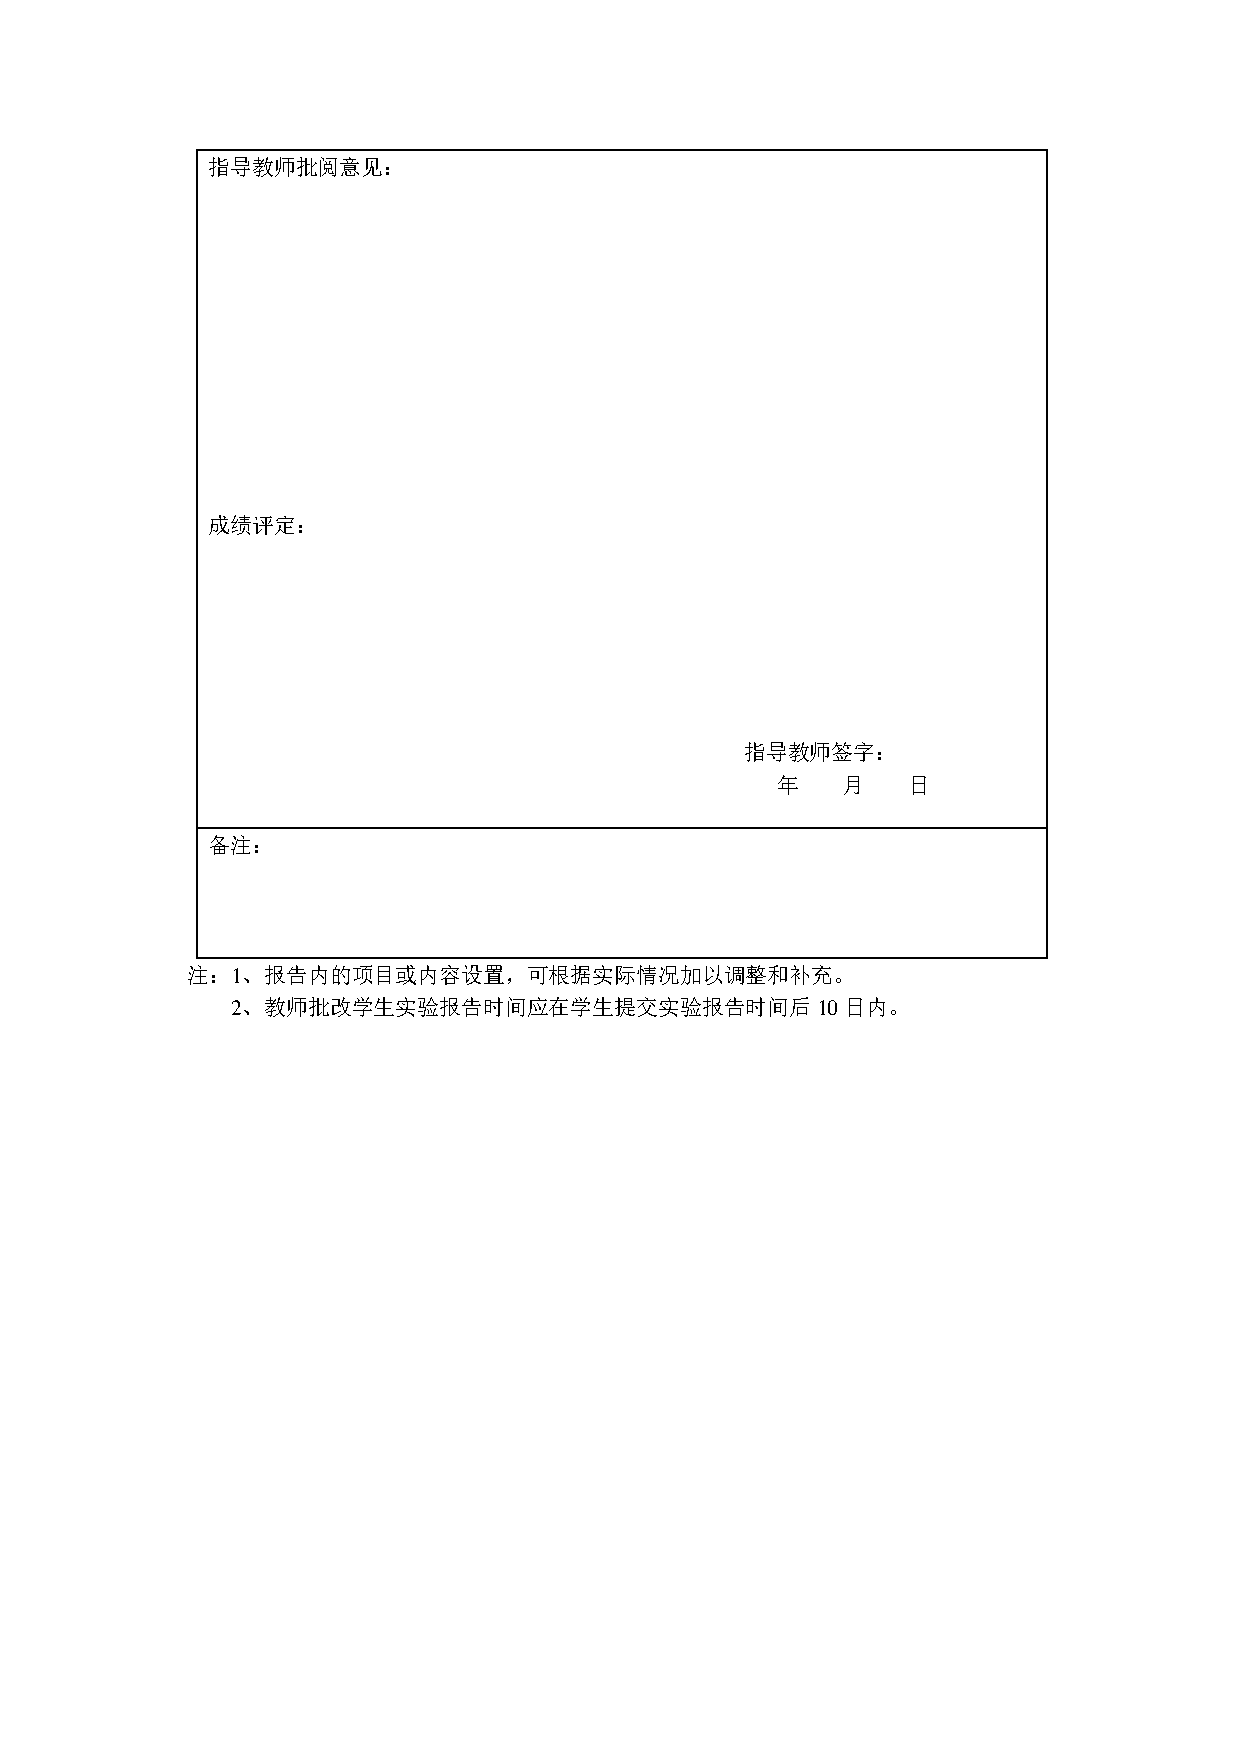
\includepdf[pages=1]{back_cover.pdf}
\end{document}
